\chapter{Signal Modelling}


\section{Hypothesis}

    The core of the Scientific method is in the practice of making a hypothesis, and of then testing that hypothesis through experiment.
    The hypothesis made in this analysis is that the Standard Model of Particle Physics is mostly correct,
        and that deviations from this theory should manifest in the probabilities of physical processes.
    I have spent the past several chapters discussing the experimentation process.
    Now it is time to discuss how I constructed a hypothesis that can be tested against the data provided from that experiment.

    The most basic hypothesis made in this analysis is simply that the di-Higgs process exists at all.
    Unfortunately, a direct measurent of the di-Higgs process is unlikely to occur in this study, as will be discussed in Chapter \ref{ch:results}.
    An additional hypothesis that can be tested however,
        relate to the Higgs Boson coupling constants and their influence on di-Higgs production cross-sections
        (recall \ref{eq:tree_level_invamp}).
    If the Standard Model is exactly correct, then the various $\kappa$ coupling constants,
        discussed in Section \ref{sec:higgs_boson},
        should all be identically 1.
    The most simple hypothesis to construct would be to calculate the expected event yield of the VBF->HH process,
        by multiplying the integrated luminosity of LHC Run 2 with the cross-section predicted by the SM.
    The same can be done to obtain predicted event yields for various alternative values of the couplings.

    \begin{table}[tbh]
       \begin{center}
           \caption{Theoretical Event yields.
                    Results retrieved via pyAMI tool~\cite{pyAMIdoc}\cite{hh4b_2021_int_note}.
                 }
           \label{tab:mcyields}
           \footnotesize
           \begin{tabular}{lllSl}
           \toprule
               \kl & \kvv & \kv & {AMI $\sigma$ [fb]} & Event Yield (for 126 fb\textsuperscript{-1}) \\
               \midrule
               1  & 1   & 1    &	1.1836  & 149.1336  \\
               1  & 0   & 1    &	18.593  & 2342.718  \\
               1  & 0.5 & 1    &	6.6177  & 833.8302  \\
               1  & 1.5 & 1    &	2.3032  & 290.2032  \\
               1  & 2   & 1    &	9.9726  & 1256.5476 \\
               1  & 3   & 1    &	44.944  & 5662.944  \\
               0  & 1   & 1    &	3.1659  & 398.9034  \\
               2  & 1   & 1    &	1.068   & 134.568   \\
               10 & 1   & 1    &	67.377  & 8489.502  \\
               1  & 1   & 0.5  &	7.5289  & 948.6414  \\
               1  & 1   & 1.5  &	45.412  & 5721.912  \\
               0  & 0   & 1    &	25.4    & 3200.4    \\
               -5 & 1   & 0.5  &	25.4    & 3200.4    \\
           \bottomrule
           \end{tabular}
       \end{center}
    \end{table}



\section{Monte-Carlo Simulation} \label{sec:mcsim}
    
    The process of simulating physics events is done in many steps, using a suit of different software programs.

    The signal simulation samples used in this analysis proceed through a production chain of three programs
        -- MadGraph, Pythia8, and Geant4 -- before going through the reconstruction and selection processes described in Chapters \ref{ch:reconstruction} and \ref{ch:selection}.

    MadGraph is used to simulate the feynman-diagram process of VBF \to HH \to 4b.
    It generates a bunch of events with output kinematics.

    Pythia8 is used to simulate particle decay, showering, and radiation.

    Geant4 simulates the entirety of the ATLAS detector.
    The particles and showers output by Pythia8 are propogated through the materials of the ATLAS machine by Geant4,
        with further showering and scattering effects modeled.
    The detectors' response to the simulated particles are recorded, with the detector output stored in the same format as that produced by the ATLAS hardware.

    \begin{table}[tbh]
       \begin{center}
           \caption{Simulated signal samples used in this analysis.
                    Results retrieved via pyAMI tool~\cite{pyAMIdoc}\cite{hh4b_2021_int_note}.
                 }
           \label{tab:mcsample}
           \footnotesize
           \begin{tabular}{lllSl}
           \toprule
               DSID  &	Type and parameters  &	Generator  &{AMI $\sigma$ [fb]}& Total gen events (MC16a+d+e) \\
               \midrule
               502970  &	VBF \kl=1, \kvv=1, \kv=1    &  MadGraph+Pythia8 &	1.1836  & $399000  +520000  +678000  $\\
               502971  &	VBF \kl=1, \kvv=0, \kv=1    &  MadGraph+Pythia8 &	18.593  & $400000  +520000  +677000  $\\
               502972  &	VBF \kl=1, \kvv=0.5, \kv=1  &  MadGraph+Pythia8 &	6.6177  & $199000  +260000  +338000  $\\
               502973  &	VBF \kl=1, \kvv=1.5, \kv=1  &  MadGraph+Pythia8 &	2.3032  & $190000  +260000  +339000  $\\
               502974  &	VBF \kl=1, \kvv=2, \kv=1    &  MadGraph+Pythia8 &	9.9726  & $199000  +258000  +213000  $\\
               502975  &	VBF \kl=1, \kvv=3, \kv=1    &  MadGraph+Pythia8 &	44.944  & $200000  +260000  +338000  $\\
               502976  &	VBF \kl=0, \kvv=1, \kv=1    &  MadGraph+Pythia8 &	3.1659  & $200000  +259000  +339000  $\\
               502977  &	VBF \kl=2, \kvv=1, \kv=1    &  MadGraph+Pythia8 &	1.068   & $200000  +259000  +323000  $\\
               502978  &	VBF \kl=10, \kvv=1, \kv=1   &  MadGraph+Pythia8 &	67.377  & $400000  +517000  +680000  $\\
               502979  &	VBF \kl=1, \kvv=1, \kv=0.5  &  MadGraph+Pythia8 &	7.5289  & $200000  +259000  +340000  $\\
               502980  &	VBF \kl=1, \kvv=1, \kv=1.5  &  MadGraph+Pythia8 &	45.412  & $200000  +259000  +340000  $\\
               502981  &	VBF \kl=0, \kvv=0, \kv=1    &  MadGraph+Pythia8 &	25.4    & $199000  +260000  +340000  $\\
               502981  &	VBF \kl=-5, \kvv=1, \kv=0.5 &  MadGraph+Pythia8 &	25.4    & $199000  +260000  +340000  $\tnote{a}\\ %FIXME
           \bottomrule
           \end{tabular}
           \begin{tablenotes}
            \item[a] 450050: This dataset was produced after the others based on the studies of Section \ref{sec:solidarity}
          \end{tablenotes}
       \end{center}
    \end{table}

\section{Signal Combination}

    As discussed in Section \ref{sec:feyn_rules}, the cross-section and kinematic distributions of the di-Higgs production processes depend fundamentally on a number of coupling constants between the Higgs and other particles.
    Of particular interest in this analysis are \kl for the Higg's self-coupling and \kvv for the \HHVV coupling.
    The values of \kl and \kvv have loose experimental constraints \cite{EXOT-2016-31} \cite{HDBS-2018-18-witherratum} \cite{ATLAS-CONF-2019-049},
        requiring analysis across a wide range of these coupling values.
    Unfortunately, the MC generation process discussed in Section \ref{sec:mcsim} is computationally expensive and time consuming.
    As such, only a handful of MC simulation samples for a select few coupling values are actually produced,
        and a sample combination technique is employed to model the signal hypothesis across the coupling parameter space.

    The process of combining a few samples in such a way as to model the entire parameter space of coupling constants is based on exploiting the underlying mathematics of the differential cross-section formula.
    By expanding the squared term of the sum of all Feynman diagram contributions,
        the cross-section can be expressed as a function of its coupling values \cite{ATLAS-CONF-2019-049}, as shown in Equation \ref{eq:tree_level_invamp}.
    Rewritting the expression again in terms of the cross-section as a function of the observable \mhh:

    \begin{equation} \begin{split} \label{eq:tree_level_invamp_simple}
        \dXsecM &\propto |\invAmp|^2 = |  \kv^2 M_t + \kv \kl M_s + \kvv M_x |^2 \\
        &\propto \kv^2 \kl^2 a_1 + \kv^4 a_2 + \kvv^2 a_3 + \kv^3 \kl a_4 + \kv \kl \kvv a_5 + \kv^2 \kvv a_6
    \end{split} \end{equation}

    The $a_i$ matrix element expansion values have a dependence on \mhh, which is not trivially derivable as an analytic function.
    Instead, for a given coupling, its cross-section for a given \mhh can be mathematically determined by solving a set of linear equations for the $a_i$ terms.
    This is done using six different cross-section values (for the same \mhh) for six different coupling values.
    In practice, the cross-section values of these six \textit{basis} samples are represented by their yields from MC simulation, binned by their \mhh.
    These six samples (rather, their \mhh-binned MC yields) are then combined using the aformentioned linear equations.
    Due to the complexities of the kinematics of the VBF process,
        the samples used in the combination must have already been run through the full reconstruction and selection process detailed in Section \ref{sec:mcsim}.
    The signal distribution modelling is thus performed by directly combining the reconstructed \mhh distributions of post-selection signal samples.

    In theory, with infinite events, the only requirement for these samples is that they are linearly independent of each other.
    In practice, the final samples are statistically limited, and different combinations of variations yield different statistical power.
    The 6-sample combination used in this analysis (\ref{tab:vbf_hh_6term_varlist} and \ref{eqn:vbf_hh_6term_chosen}) has been chosen specifically for its ability to avoid mismodelling errors.

    \begin{table}[] \centering
    \caption{6-Term VBF Combination Sample Variations}
    \label{tab:vbf_hh_6term_varlist}
    \begin{tabular}{ |l|l|l| }
        \hline
        \textbf {$\kappa_{2V}$} & \textbf {$\kappa_\lambda$} & \textbf {$\kappa_V$} \\
        \hline
            1   &   1 & 1   \\
            1.5 &   1 & 1   \\
            1   &   2 & 1   \\
            1   &  10 & 1   \\
            1   &   1 & 0.5 \\
            0   &  -5 & 0.5 \\
        \hline
    \end{tabular} \end{table}

    \begin{equation}
    \label{eqn:vbf_hh_6term_chosen}
    \begin{split}
        \frac{d\sigma}{d\mhh}(\kvv, \kl, \kv) =
            \left(\frac{68 \kappa_{2V}^{2}}{135} - 4 \kappa_{2V} \kappa_{V}^{2} + \frac{20 \kappa_{2V} \kappa_{V} \kappa_{\lambda}}{27} + \frac{772 \kappa_{V}^{4}}{135} - \frac{56 \kappa_{V}^{3} \kappa_{\lambda}}{27} + \frac{\kappa_{V}^{2} \kappa_{\lambda}^{2}}{9}\right) \times \frac{d\sigma}{d\mhh}{\left(1,1,1 \right)} \\
            + \left(- \frac{4 \kappa_{2V}^{2}}{5} + 4 \kappa_{2V} \kappa_{V}^{2} - \frac{16 \kappa_{V}^{4}}{5}\right) \times \frac{d\sigma}{d\mhh}{\left(\frac{3}{2},1,1 \right)} \\
            + \left(\frac{11 \kappa_{2V}^{2}}{60} + \frac{\kappa_{2V} \kappa_{V}^{2}}{3} - \frac{19 \kappa_{2V} \kappa_{V} \kappa_{\lambda}}{24} - \frac{53 \kappa_{V}^{4}}{30} + \frac{13 \kappa_{V}^{3} \kappa_{\lambda}}{6} - \frac{\kappa_{V}^{2} \kappa_{\lambda}^{2}}{8}\right) \times \frac{d\sigma}{d\mhh}{\left(1,2,1 \right)} \\
            + \left(- \frac{11 \kappa_{2V}^{2}}{540} + \frac{11 \kappa_{2V} \kappa_{V} \kappa_{\lambda}}{216} + \frac{13 \kappa_{V}^{4}}{270} - \frac{5 \kappa_{V}^{3} \kappa_{\lambda}}{54} + \frac{\kappa_{V}^{2} \kappa_{\lambda}^{2}}{72}\right) \times \frac{d\sigma}{d\mhh}{\left(1,10,1 \right)}  \\
            + \left(\frac{88 \kappa_{2V}^{2}}{45} - \frac{16 \kappa_{2V} \kappa_{V}^{2}}{3} + \frac{4 \kappa_{2V} \kappa_{V} \kappa_{\lambda}}{9} + \frac{152 \kappa_{V}^{4}}{45} - \frac{4 \kappa_{V}^{3} \kappa_{\lambda}}{9}\right) \times \frac{d\sigma}{d\mhh}{\left(1,1,\frac{1}{2} \right)} \\
            + \left(\frac{8 \kappa_{2V}^{2}}{45} - \frac{4 \kappa_{2V} \kappa_{V} \kappa_{\lambda}}{9} - \frac{8 \kappa_{V}^{4}}{45} + \frac{4 \kappa_{V}^{3} \kappa_{\lambda}}{9}\right) \times \frac{d\sigma}{d\mhh}{\left(1,-5,\frac{1}{2} \right)}
    \end{split}
    \end{equation}

    The method used to determine the overall performance of a basis is to check the number of negative bins generated
        in the \mhh distribution across all points in the two-dimensional \kvv,\kl space, as seen in \ref{fig:vbf_hh_6term_nWeight_grid}.
    As negative bin weights are unphysical, they indicate poor signal modelling.
    Thus, identifying a basis which minimizes the presence of negative weights ensures stable modeling of the signal hypothesis at all points in the coupling space (\ref{fig:vbf_hh_6term_validation} and \ref{fig:vbf_hh_6term_preview}).

    \begin{figure}[tbh]
        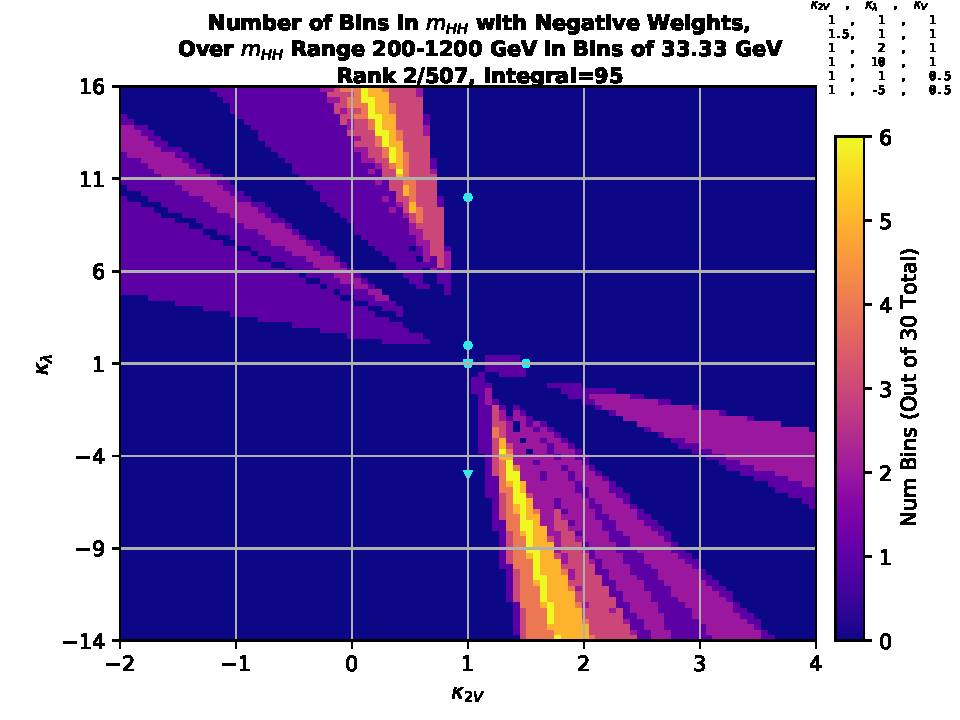
\includegraphics[width=\linewidth,height=\textheight,keepaspectratio]{signal/negative_weights_base}
        \caption{
            Frequency of negative bin weights in \mhh distribution across \kvv,\kl range.
            Brighter regions indicate more negative-weighted bins, and suggest less stable signal modelling.
            This particular combination of samples was chosen for how much of the space is ``dark",
                with darker regions indicating generally stable signal modelling.
            The table of coupling values in the upper right corner indicates the 6 MC samples
                (highlighted on the plot with cyan dots) used in the combination.
        }
        \label{fig:vbf_hh_6term_nWeight_grid}
    \end{figure}

    Ultimately however, the final arbiter of a well constructed basis is that it produces observable distributions comparable to what would be produced through direct MC generation.
    A number of validation tests are thus performed, comparing the distributions from the combination to an already existing MC sample.
    Displayed in Figure \ref{fig:vbf_hh_6term_validation}, the combination shows strong agreement with the MC sample.

    \begin{figure}[tbh]
        \subfloat[Validation \kv = 1.5]{
            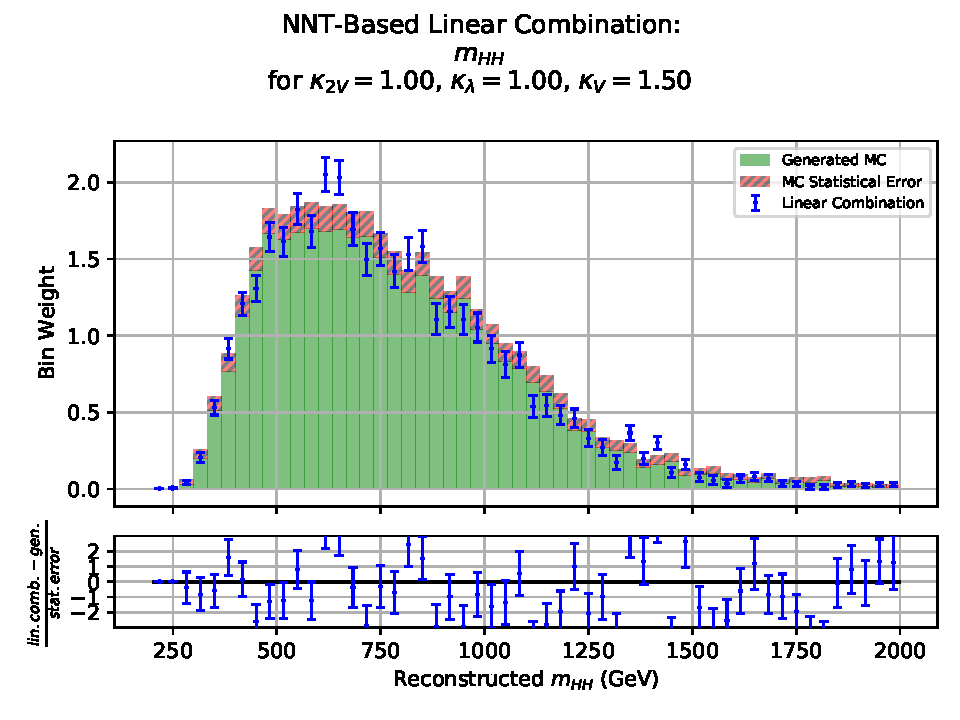
\includegraphics[width=0.5\linewidth,height=\textheight,keepaspectratio]{signal/reco_mHH_cvv1p00cl1p00cv1p50}
        }
        \subfloat[Validation \kl = 0]{
            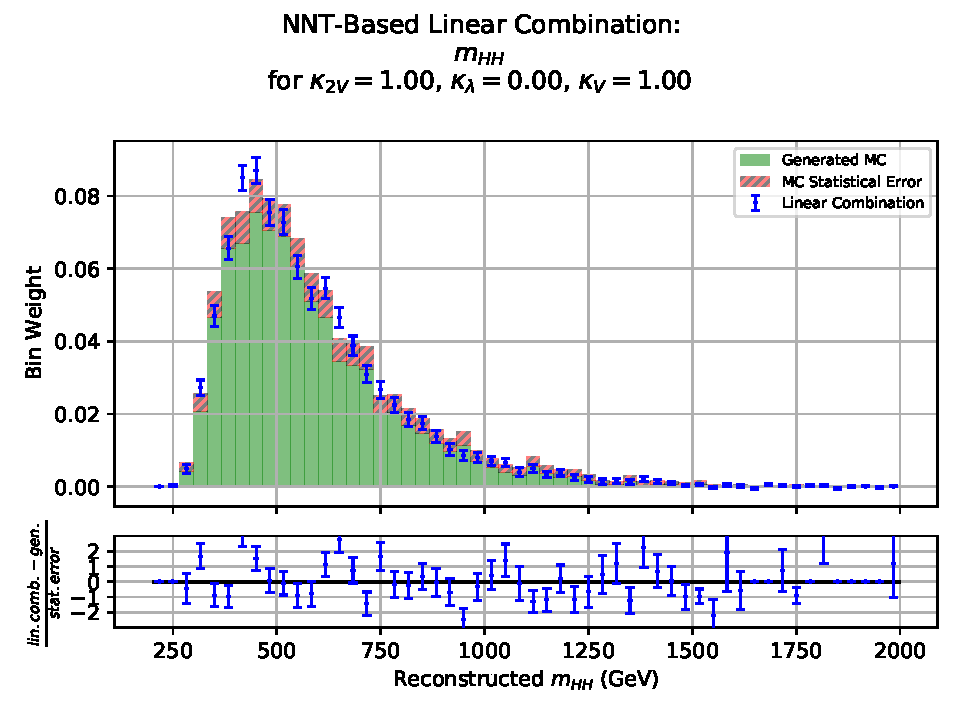
\includegraphics[width=0.5\linewidth,height=\textheight,keepaspectratio]{signal/reco_mHH_cvv1p00cl0p00cv1p00}
        }
        \caption{
            Validation of 6-term combination against MC generated at \kv = 1.5 and \kl = 0.
            The combination shows good agreement to the generated MC distributions.
        }
        \label{fig:vbf_hh_6term_validation}
    \end{figure}

    \begin{figure}[tbh]
    	\centering
        \subfloat[Validation against MC with $\kl=0$]{
            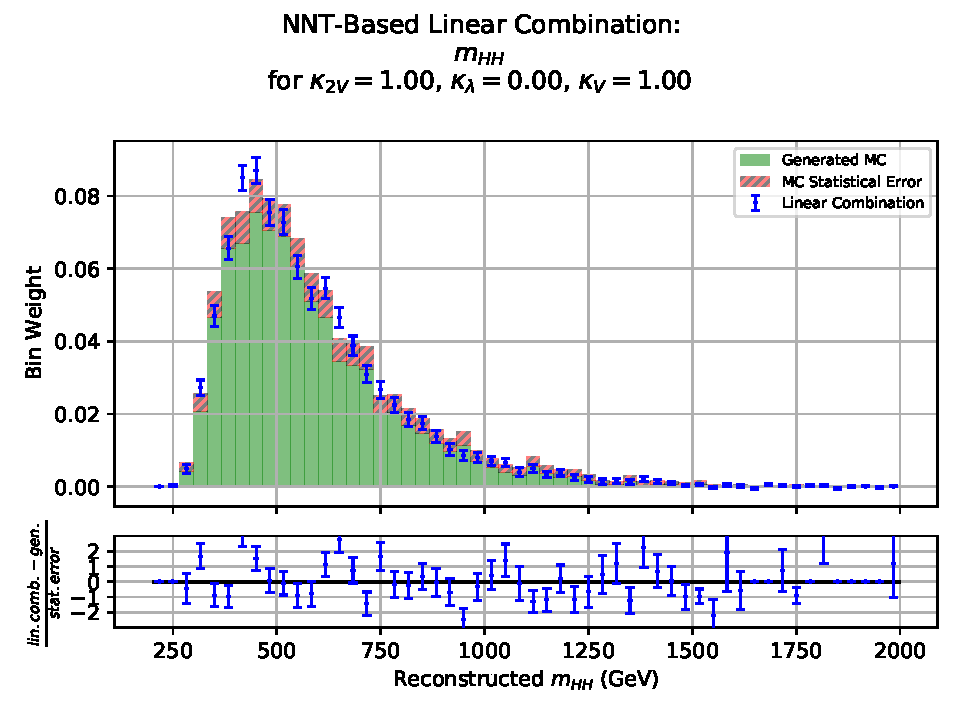
\includegraphics[width=0.32\linewidth,height=\textheight,keepaspectratio]{signal/reco_mHH_cvv1p00cl0p00cv1p00}
        }
        \subfloat[Validation against MC with $\kvv=0$]{
            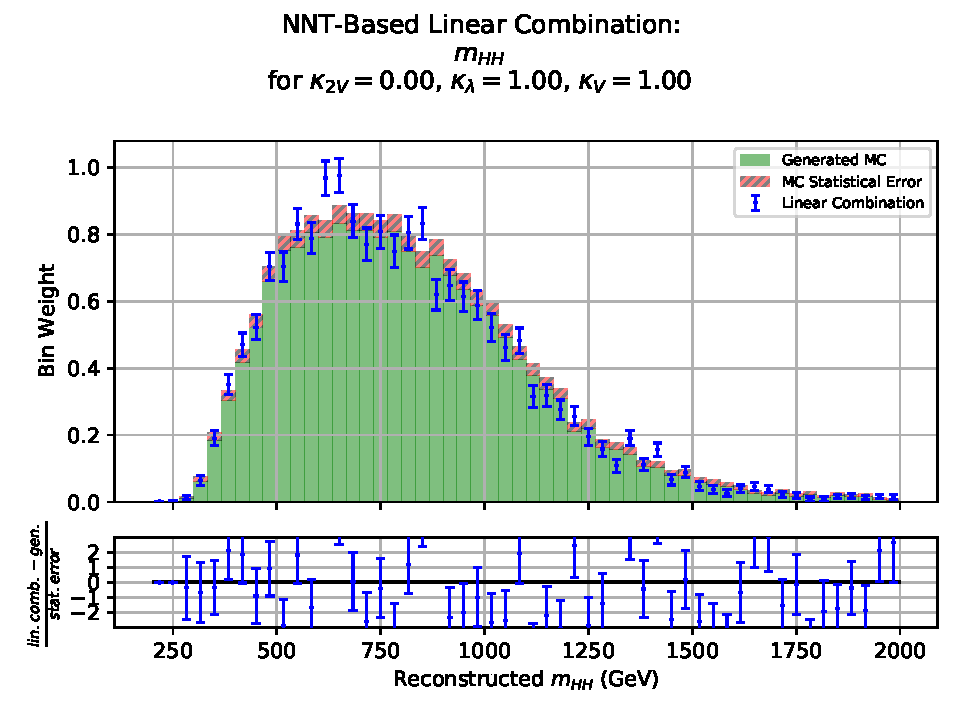
\includegraphics[width=0.32\linewidth,height=\textheight,keepaspectratio]{signal/reco_mHH_cvv0p00cl1p00cv1p00}
        }
        \subfloat[Validation against MC with $\kvv=3$]{
            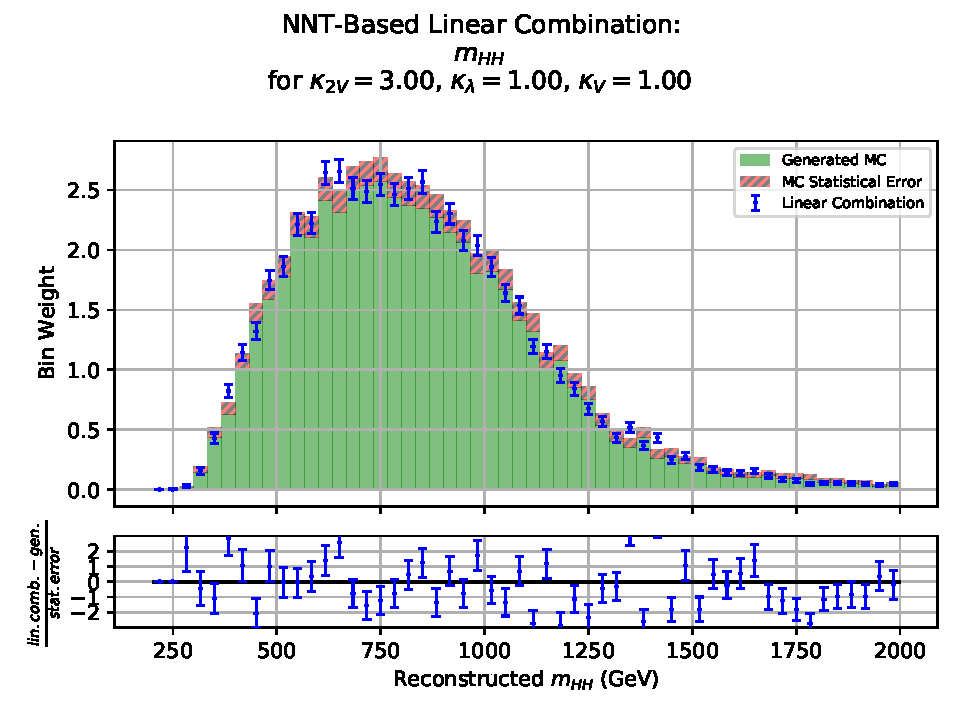
\includegraphics[width=0.32\linewidth,height=\textheight,keepaspectratio]{signal/reco_mHH_cvv3p00cl1p00cv1p00}
        }
        \caption{
            The six-term linear combination of samples is combined for various coupling values.
            The combined distribution shape (in blue) is compared against a Monte-Carlo sample (in green) which was generated for the same coupling values.
            The combination approach shows good agreement with the generated sample, indicating accurate modelling of the signal shape.
        }
        \label{fig:vbf_hh_validation}
    \end{figure}

    As an additional test, I also checked the distribution shape predicted by the combination at points far from the SM.
    These points have no MC samples to compare to, but the points can still be checked to ensure they at least look well-behaved.

    \begin{figure}[tbh]
        \centering
        \subfloat[Combined \mhh distribution at \kvv = 2.5, \kl = -10]{
            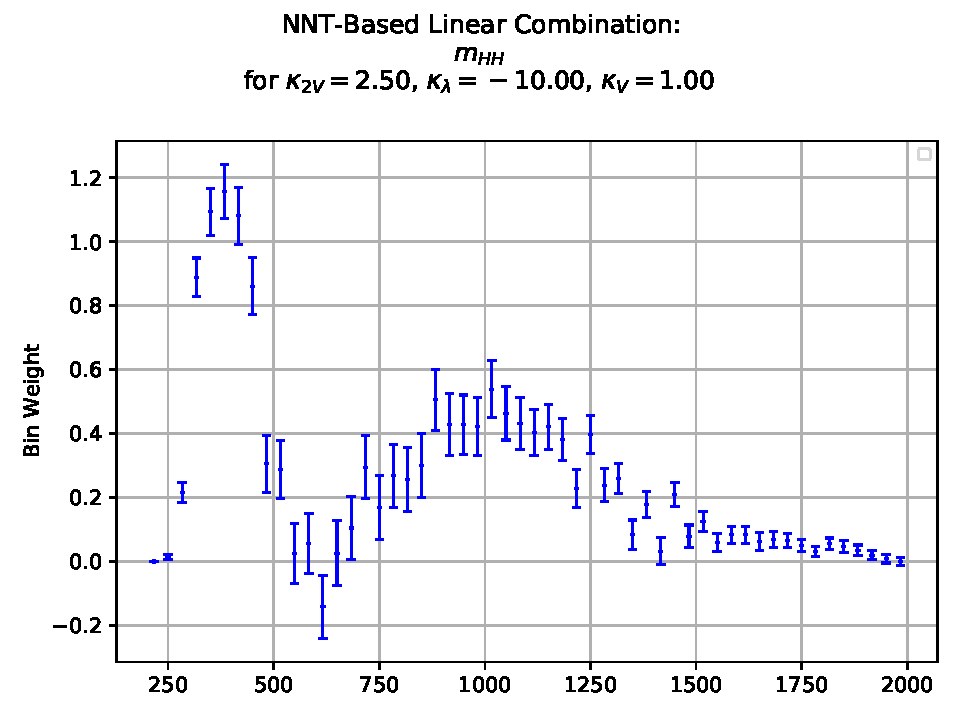
\includegraphics[width=0.32\linewidth,height=\textheight,keepaspectratio]{signal/preview_reco_mHH_new_cvv2p50cl-10p00cv1p00}
        }
        \subfloat[Combined \mhh distribution at \kvv = 2.0, \kl = -10]{
            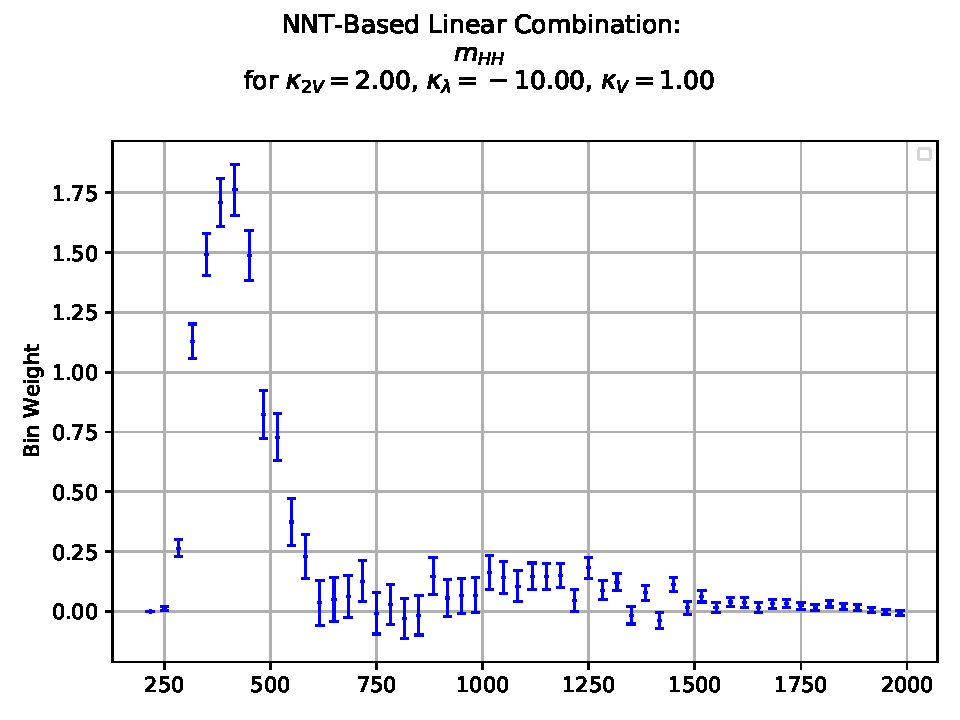
\includegraphics[width=0.32\linewidth,height=\textheight,keepaspectratio]{signal/preview_reco_mHH_new_cvv2p00cl-10p00cv1p00}
        }
        \subfloat[Combined \mhh distribution at \kvv = 0, \kl = 13]{
            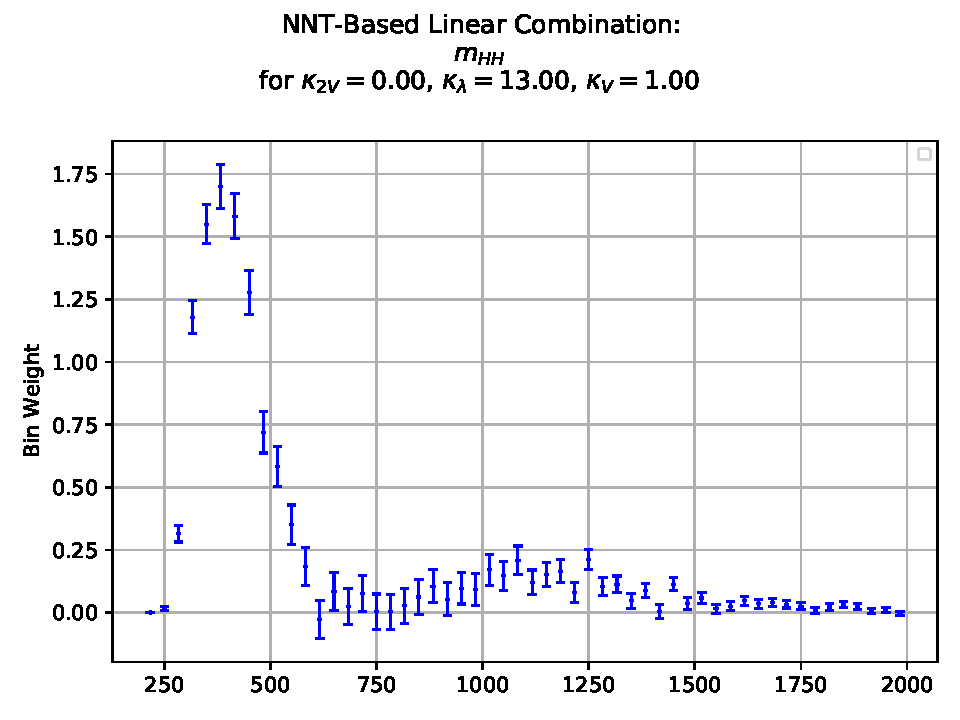
\includegraphics[width=0.32\linewidth,height=\textheight,keepaspectratio]{signal/preview_reco_mHH_new_cvv0p00cl13p00cv1p00}
        }
        \caption{
            \mhh distribution produced by the 6-term combination at points far from the SM.
            The combination produces smooth, well-behaved distributions at these points,
                suggesting the signal is well-modelled in these regions.
        }
        \label{fig:vbf_hh_6term_preview}
    \end{figure}

    \begin{figure}[tbh]
    	\centering
        \subfloat[Combination at  \kvv = -2]{
            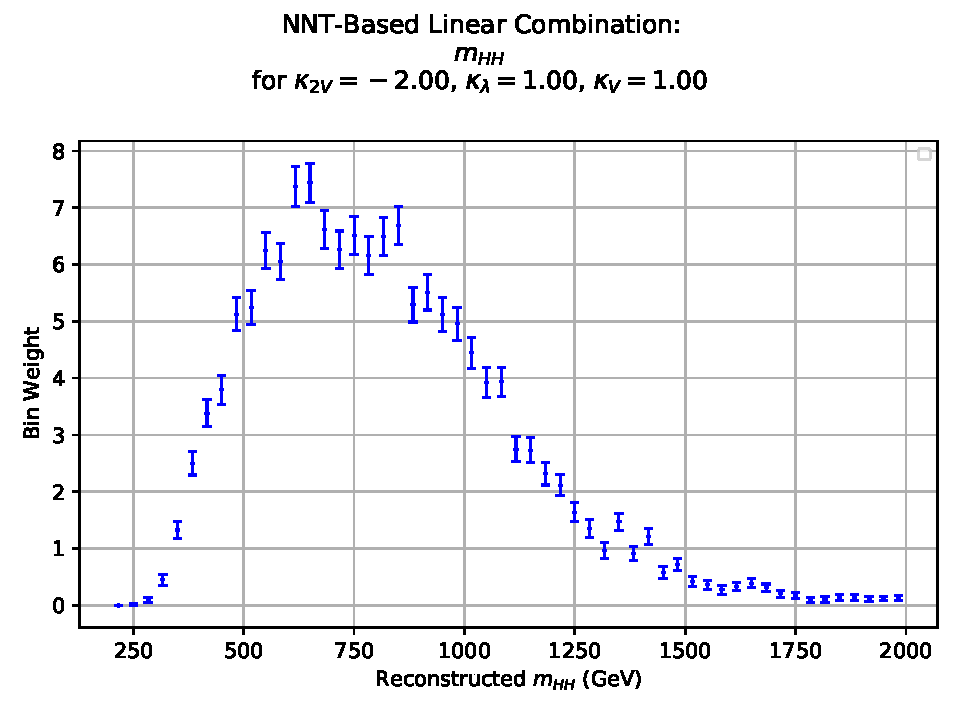
\includegraphics[width=0.44\linewidth,height=\textheight,keepaspectratio]{signal/preview_reco_mHH_new_cvv-2p00cl1p00cv1p00}
        }
        \subfloat[Combination at  \kl = -9]{
            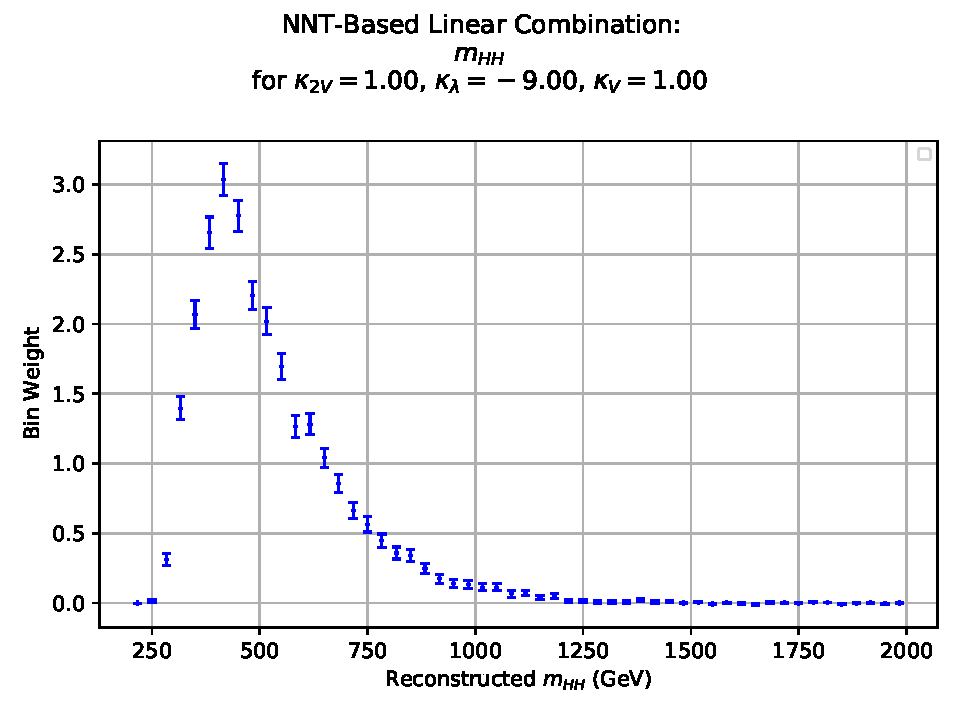
\includegraphics[width=0.44\linewidth,height=\textheight,keepaspectratio]{signal/preview_reco_mHH_new_cvv1p00cl-9p00cv1p00}
        }
        \caption{
            The six-term linear combination of samples is combined for coupling values very far from the Standard Model.
            There are no MC simulated samples to compare these points too, but the combined distributions at these points are smooth and well-behaved,
                indicating reasonable modelling of the distribution even at distant couplings.
        }
        \label{fig:vbf_hh_preview}
    \end{figure}


\section{Solidarity} \label{sec:solidarity}
    
    As a final note on the discussion of the signal sample combination technique,
        I would like to address the reason that some combination bases work better than others.
    Originally, the 2021 MC production for the 4b analysis consisted of 12 samples (All but the bottom row of Table \ref{tab:mcsample}).
    However, inspection of these samples using the Negative Weight technique discussed above revealed very poor modeling performance.
    From a combinatorics perspective, there were 12 samples available, and six are needed for the combination.
    There are 924 ways to choose 6 samples from 12, and of those 619 produce linearly solvable systems of equations.
    Of the 619, only 250 include the Standard Model MC sample.
    None of these 250 combination bases produced stable signal models across the $\kappa$-coupling space.
    The performance of the two bases with the overall fewest number of negative bin weights is shown in Figures \ref{fig:mcnWeight_old} and \ref{fig:mcpreviews_old}.

    \begin{figure}[tbh]
    	\centering
        \subfloat[Original 12, Rank 1 Negative Weight Heatmap]{ 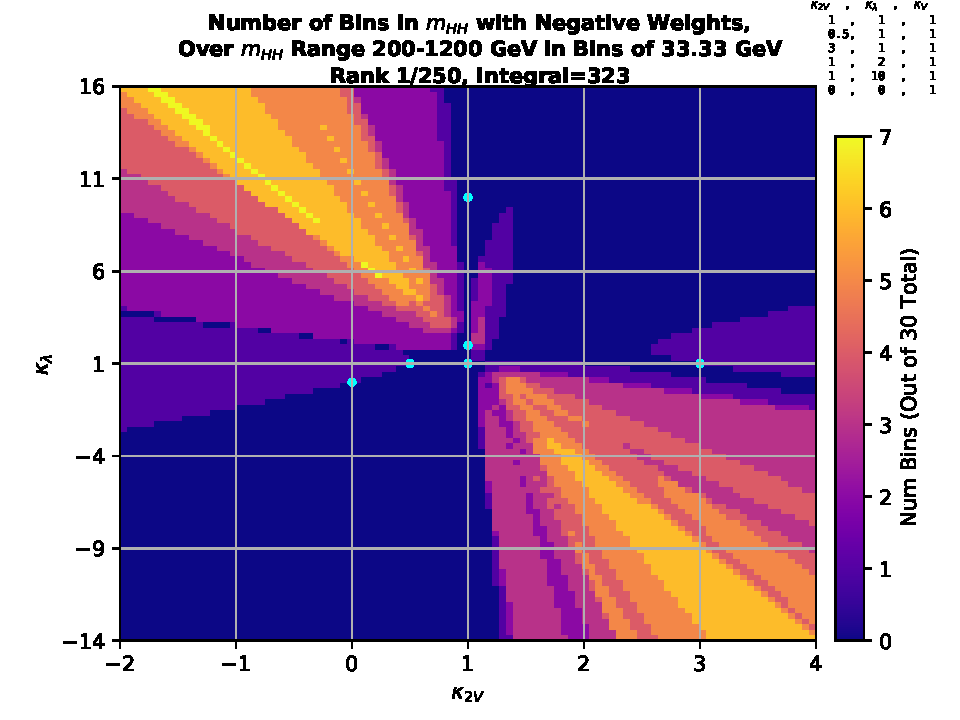
\includegraphics[width=0.44\linewidth,height=\textheight,keepaspectratio]{signal/negative_weights_toprank0} }
        \subfloat[Original 12, Rank 2 Negative Weight Heatmap]{ 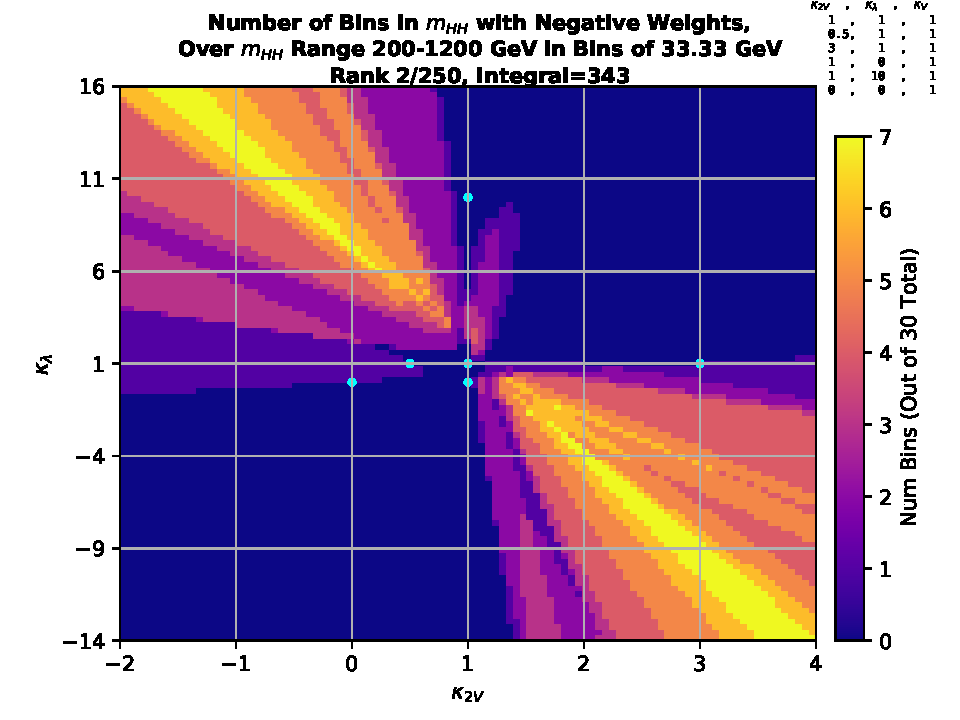
\includegraphics[width=0.44\linewidth,height=\textheight,keepaspectratio]{signal/negative_weights_toprank1} }
        \caption{
            The two best performing bases of the original 12 MC samples.
            Both bases show a distressing abundance of negative weighted bins across a wide swath of the $\kappa$-couplings space.
        }
        \label{fig:mcnWeight_old}
    \end{figure}


    \begin{figure}[tbh]
    	\centering
        \subfloat[]{ 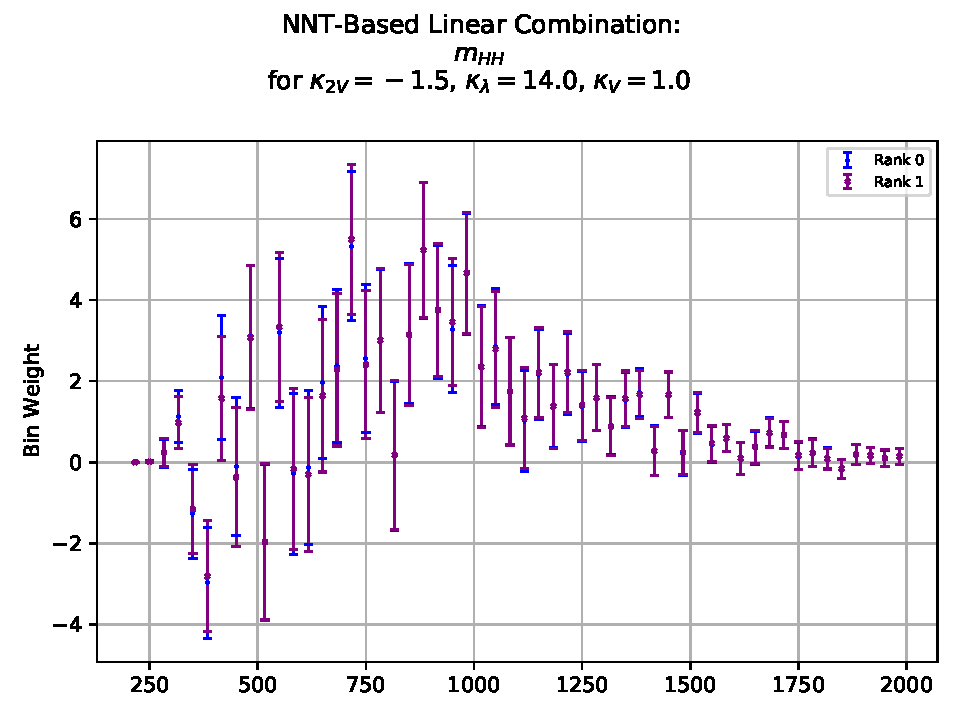
\includegraphics[width=0.44\linewidth,height=\textheight,keepaspectratio]{signal/reco_mHH_compare_preview_auto_top_3D_0-1_cvv-1p5cl14p0cv1p0} }
        \subfloat[]{ 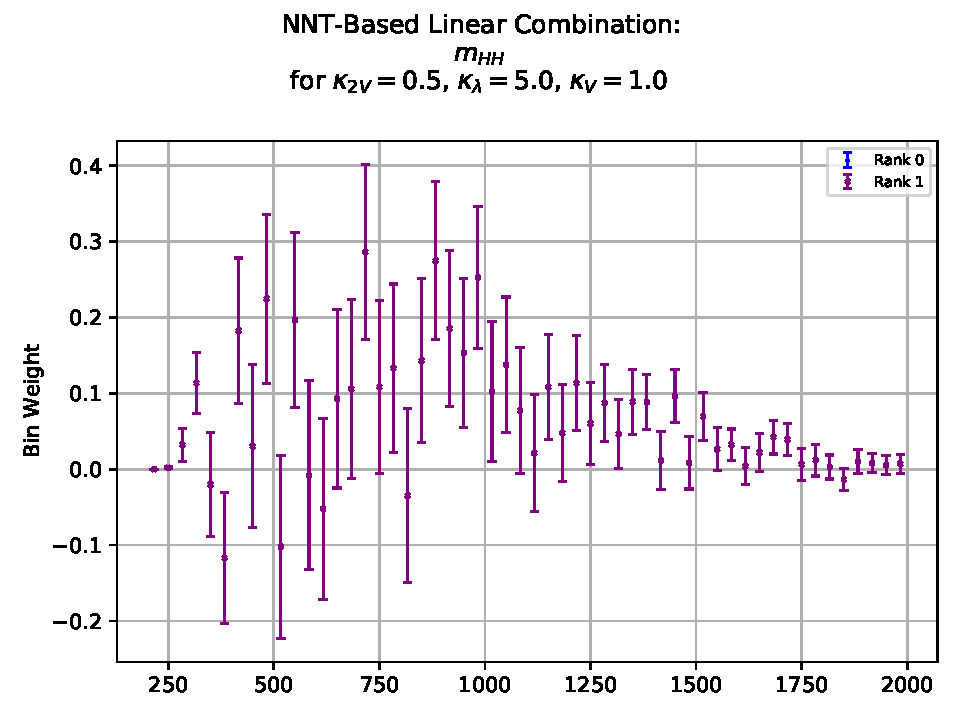
\includegraphics[width=0.44\linewidth,height=\textheight,keepaspectratio]{signal/reco_mHH_compare_preview_auto_top_3D_0-1_cvv0p5cl5p0cv1p0} }\\
        \subfloat[]{ 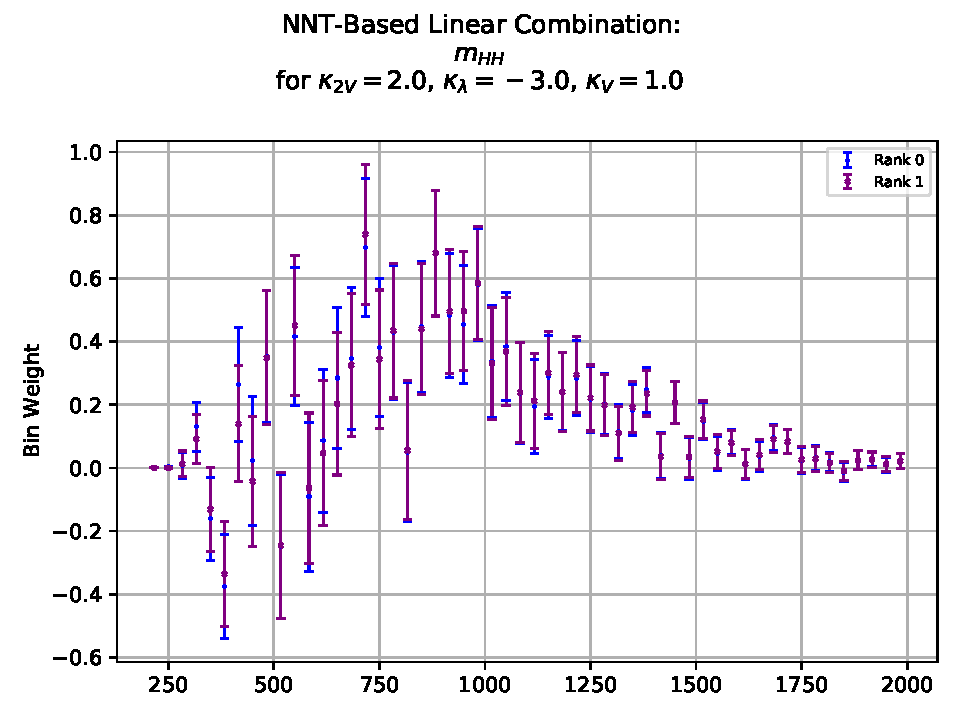
\includegraphics[width=0.44\linewidth,height=\textheight,keepaspectratio]{signal/reco_mHH_compare_preview_auto_top_3D_0-1_cvv2p0cl-3p0cv1p0} }
        \subfloat[]{ 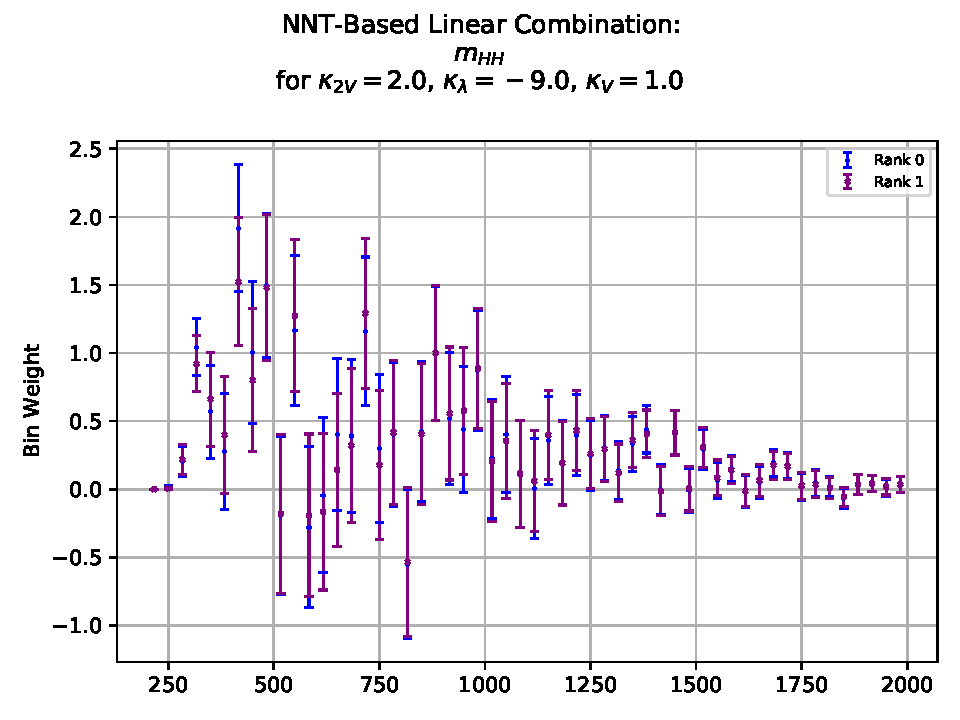
\includegraphics[width=0.44\linewidth,height=\textheight,keepaspectratio]{signal/reco_mHH_compare_preview_auto_top_3D_0-1_cvv2p0cl-9p0cv1p0} }
        \caption{
            The two best performing bases of the original 12 MC samples,
                modelling \mhh distributions for points far from the SM.
            Both bases produce very unstable distributions.
        }
        \label{fig:mcpreviews_old}
    \end{figure}


    The proposed solution was to generate one additional MC sample,
        which could be used in combination with five of the original samples to produce a stable basis.
    Of course, until the sample was produced, the negative weight optimization technique could not be used to asses the new sample's performance.
    As such, I developed a novel optimization metric which could predict the performance of a particular basis,
        without the need for any MC production.
    My hypothesis for the behaviour of the sample combinations is that the regions of the coupling space which perform poorly
        (e.g.\ the top left corners of Figure \ref{fig:mcnWeight_old}),
        do so because one or two of the samples is disproportionately represented in the combination compared to the others.
    The formula for the combination of the samples amounts to weighting each sample's yield by a coupling-dependent coefficient,
        and then adding these weighted yields together to obtain the combined yield.
    Different samples can have yields which are orders of magnitude different from each other
        (e.g./ the 1.18 fb yield of the SM point to the 67 fb yield of the \kl=10 sample).
    As well, the coupling-based coefficients can vary dramatically across the coupling space.
    The product of the sample yield and the coupling coefficient (the \textit{weighted yield})
        can therefore vary a great deal across the coupling space.
    For many regions of the coupling space, it can happen that one or two of the samples' weighted yields vastly outweigh the others.
    In such cases, the combined yield is then based almost entirely on these one or two over-represented samples,
        making the combination much more susceptible to statistical deficiencies.
    I propose that this ``closeness'' of the weighted yields can be used as a highly effective metric of performance,
        and one which does not neccesarily depend on the generation of MC.

    Here I define a metric to quantify this behaviour.
    Due to the nature of the weighted yields,
        the metric will be dependant both on the basis samples' yields ($\sigma_i$),
        and on the coupling coefficient ($c_i(\kvv,\kl,\kv)$) of the specific point in the coupling space to be modeled.
    As well, I want to explicitly note the occurance of \textit{negative} coefficients in the combination sum.
    I propose that negative coefficients are \textit{not} intrinsically a bad thing.
    Rather, they merely reflect the behaviour inherent in calculating cross-sections,
        in that some Feynman diagrams invariably cancel with others.
    Thus, I will be looking at the ``closeness'' of the \textit{absolute values} of the weighted yields,
        specifically ensuring that bases are \textbf{not} penalized for large cancellations between terms.
    The resulting metric, which I deem \textit{Solidarity}, effectively measures how well the basis samples work together at a given point.

    \begin{equation}
    \textrm{\textbf{Solidarity}: }S \equiv \frac{ \sum\limits_{i=1}^6 c_i\sigma_i }{ \textrm{Stdev}(|c_i\sigma_i|) }
    \end{equation}

    That is, first take the standard deviation of the absolute values of the $c_i\sigma_i$ weighted yields.
    Normalize this by the combined yield at that point (i.e.\ the sum of the weighted yields).
    Then take the \textit{reciprocal} of this normalized standard deviation,
        such that $S$ increases as the absolute standard deviation gets smaller.
    The quantity used for the samples' yields can vary,
        but the advantage of Solidarity as a metric
        is that yield can be represented by the pure theoretical cross-section.
    So long as the process of reconstruction and selection does not alter the ratios of the various samples' total event yields,
        this allows Solidarity to be used to gauge the performance of a basis without the need for any MC production.

    As the metric is calculated on a per-coupling basis,
        a heatmap similar to the Negative Weight Heatmap can be generated in a similar manner.

    \begin{figure}[tbh]
    	\centering
        \subfloat[]{ 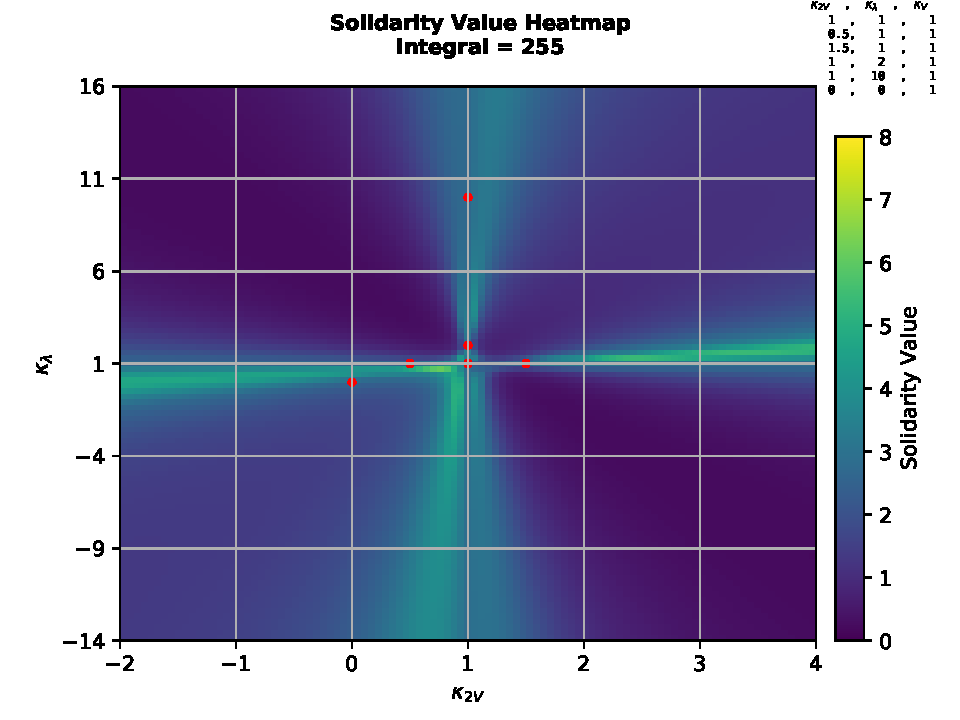
\includegraphics[width=0.5\linewidth,height=\textheight,keepaspectratio]{signal/solidarity_main_rank00old} }
        \subfloat[]{ 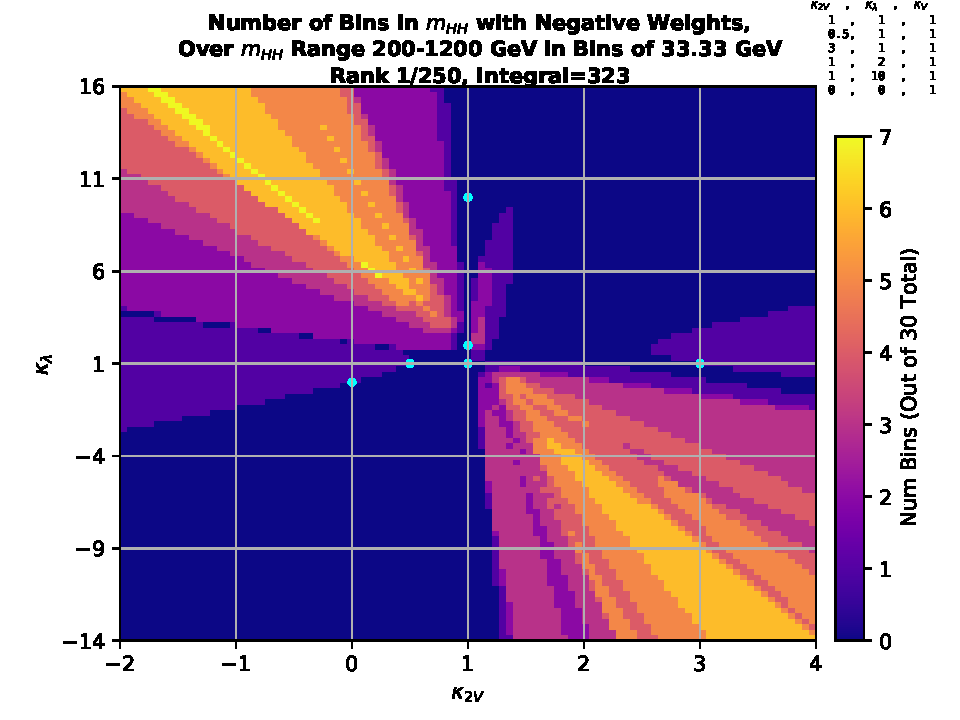
\includegraphics[width=0.5\linewidth,height=\textheight,keepaspectratio]{signal/negative_weights_toprank0} }\\
        \subfloat[]{ 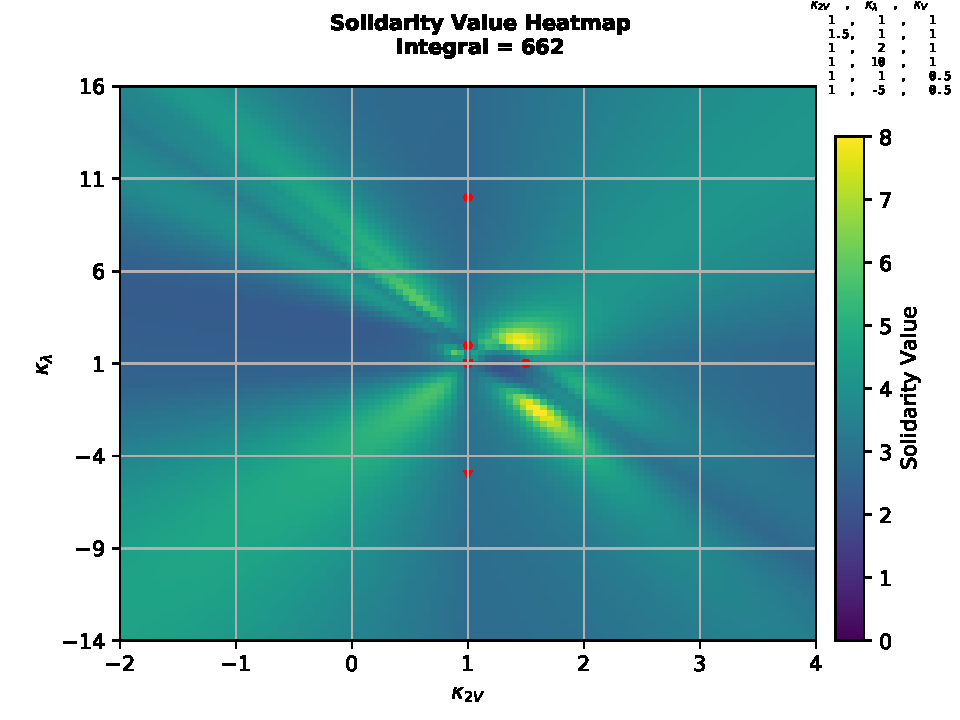
\includegraphics[width=0.5\linewidth,height=\textheight,keepaspectratio]{signal/solidarity_main_rank01} }
        \subfloat[]{ 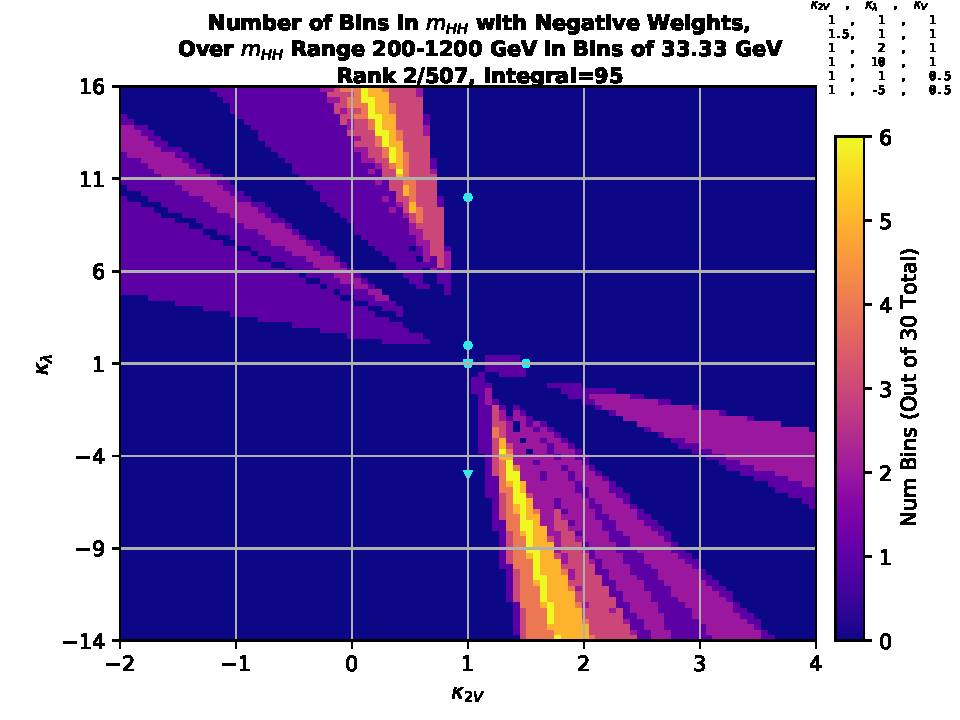
\includegraphics[width=0.5\linewidth,height=\textheight,keepaspectratio]{signal/negative_weights_base} }
        \caption{
            The heatmap of Solidarity calculated with theoretical cross-section values (left),
                compared to the Negative Weight Heatmap generated by the post-reconstruction and selection MC samples (right).
            The top two plots correspond to the \textit{original} optimal basis (before the inclusion of the 13th sample),
                while the bottom two correspond to the optimal basis sample used in the analysis.
            Note that the regions of low Solidarity values correspond strongly to the regions with large numbers of negative-weighted bins.
            Also note the ``Integral'' values of the different bases (shown just below their titles).
        }
        \label{fig:solidarity_heatmaps}
    \end{figure}

    The map of Solidarity (Figure \ref{fig:solidarity_heatmaps}) shows a strong relationship with the prevalence of negative-weighted bins,
        despite the Solidarity heatmap being calculated without the use of any MC simulation samples.
    Using the surface integral of the heatmap as was done for the negative-weight map allows a similar metric to be given to a basis as a whole.
    Comparing this Theoretical Solidarity Integral to the corresponding Negative Weight Integral (Figure \ref{fig:nWeight_solidarity_scatter})
        shows a very strong correlation between the two,
        which can be exploited to predict useful samples bases before generating any MC samples.

    \begin{figure}[tbh]
        \subfloat[Original 12 Samples]{ 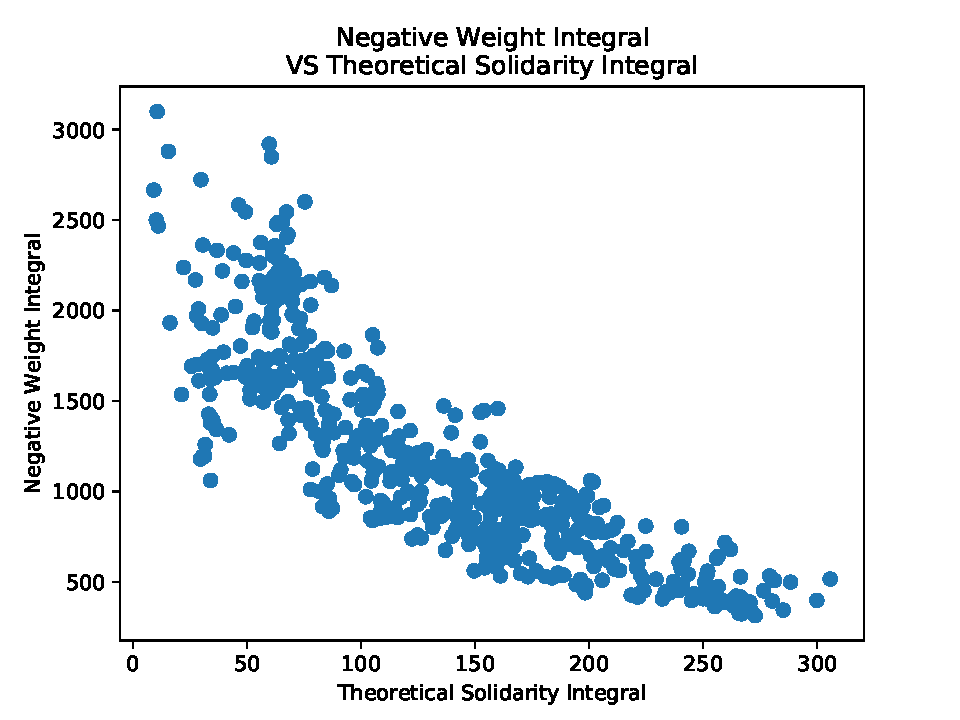
\includegraphics[width=0.5\linewidth,height=\textheight,keepaspectratio]{signal/Nweight_integral_VS_theory_solidarity_integral_old} }
        \subfloat[Using All 13 Samples]{ 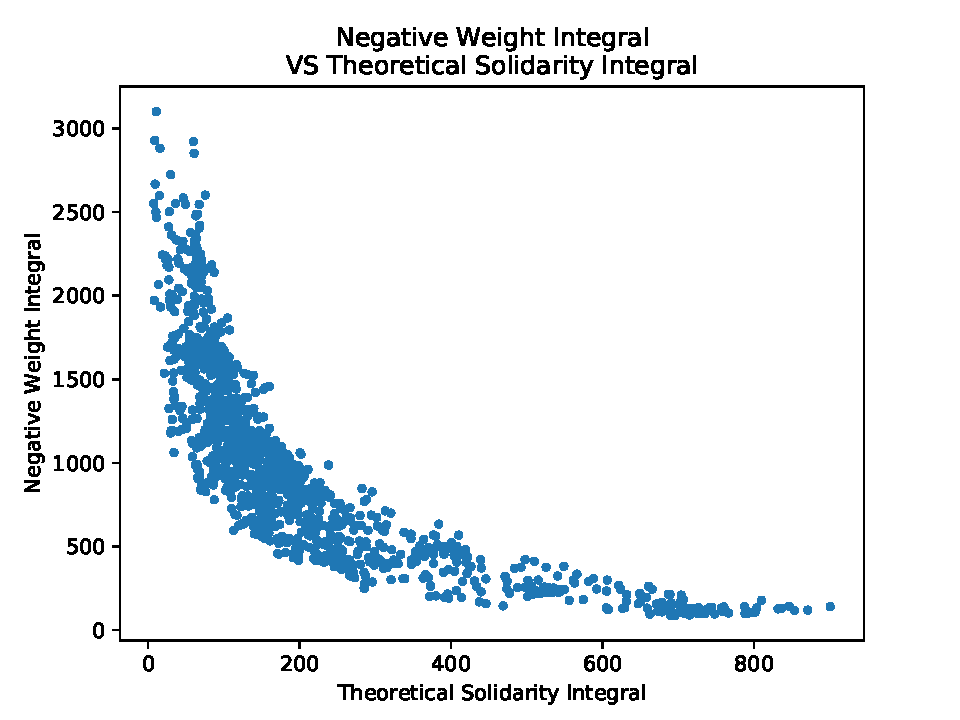
\includegraphics[width=0.5\linewidth,height=\textheight,keepaspectratio]{signal/Nweight_integral_VS_theory_solidarity_integral} }
        \caption{
            Plots of the Negative Weight Surface Integral (calculated from post-reconstruction/selection MC samples)
                of all possible bases, with respect to the same bases' Solidarity Surface Integral
                (calculated from the theoretical cross-section associated with the MC samples' coupling values).
            The plot on the left uses only the original 12 available MC samples for its bases.
            To the right is the same plot with the inclusion of the 13th (\kl=-5, \kvv=1, \kv=0.5) sample.
            Note that the plot on the left has a y-axis with a lower bound that is significantly higher (~ 250) 
                than the full-13-sample plot (lower bound ~100),
                indicating the presence of more optimal bases afforded by the 13th sample.
        }
        \label{fig:nWeight_solidarity_scatter}
    \end{figure}


    Figure \ref{fig:nWeight_solidarity_scatter} was generated using all 1307 linearly independant bases of combining 6 of the 13 available MC samples.
    Due to the strong correlation between negative-weighted bins and solidarity,
        a histogram of only the Theoretical Solidarity Surface Integral
        (effectively just the x-axis of Figure \ref{fig:nWeight_solidarity_scatter})
        can be used to determine the overall potential performance a set of MC samples might have.
    In order to determine which MC sample should be produced to work most effectively with the already existing 12 samples,
        I constructed such Solidarity Surface Integral histograms for a wide range of possible new samples.
    Each histogram was constructed using the bases formed from all possible combinations of 6 samples from
        the 12 original samples plus one prospective MC sample.
    Thus, each Solidarity Surface Integral histogram corresponded to 13 samples,
        and served as a figure of merit for the 13th (the prospective) sample's performance.

    \begin{figure}[tbh]
        \subfloat[Original 12 Samples]{
            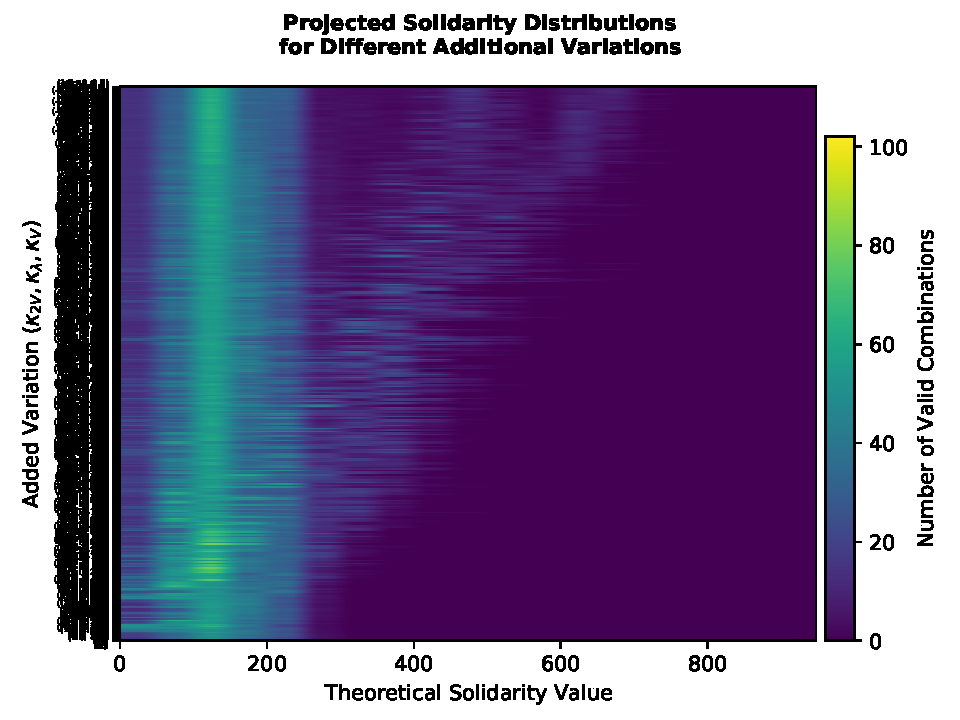
\includegraphics[width=0.5\linewidth,height=\textheight,keepaspectratio]{signal/projective_solidarity_all}
        }
        \subfloat[Using All 13 Samples]{
            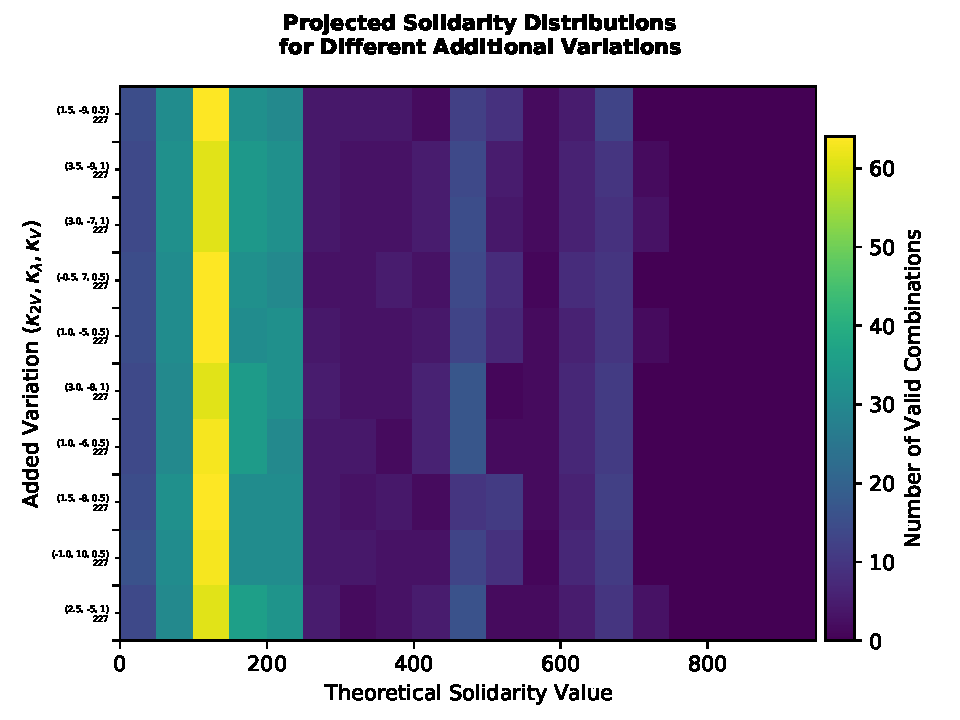
\includegraphics[width=0.5\linewidth,height=\textheight,keepaspectratio]{signal/projective_solidarity_dump}
        }
        \caption{
            plot of all the histograms.
            The rows are sorted from top to bottom by the sum of their bins
                (That is, the sum of all Solidarity surface integrals for all bases associated with the same additional MC sample point).
        }
        \label{fig:solidarity_dump}
    \end{figure}

    Aligning all of these histograms together as in Figure \ref{fig:solidarity_dump}
        produces a clear method of distinguishing samples that 
        could produce high stability combinations with the existing 12 samples.
    The aggregate sum of all Solidarity surface integrals associated with a new sample
        can evidently be used as a scalar metric to by which to rank different prospective coupling points.
    The culmination of these tests is Figure \ref{fig:solidarity_performance_map}

    \begin{figure}[tbh]
        \subfloat[\kv = 1]{
            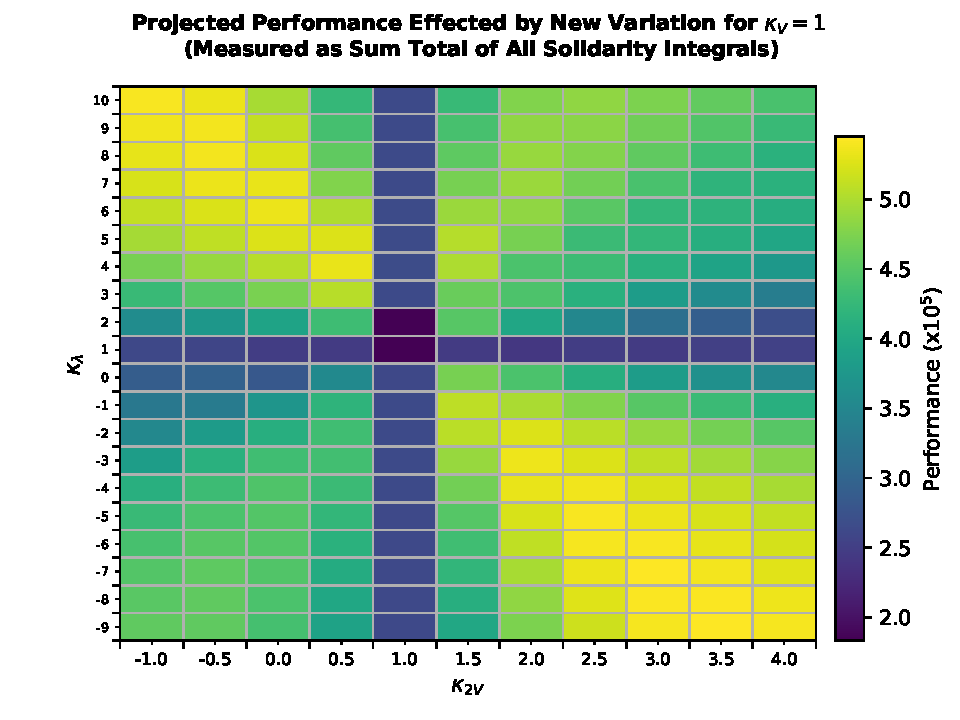
\includegraphics[width=0.5\linewidth,height=\textheight,keepaspectratio]{signal/solidarity_performance_kv1}
        }\\
        \subfloat[\kv = 0.5]{
            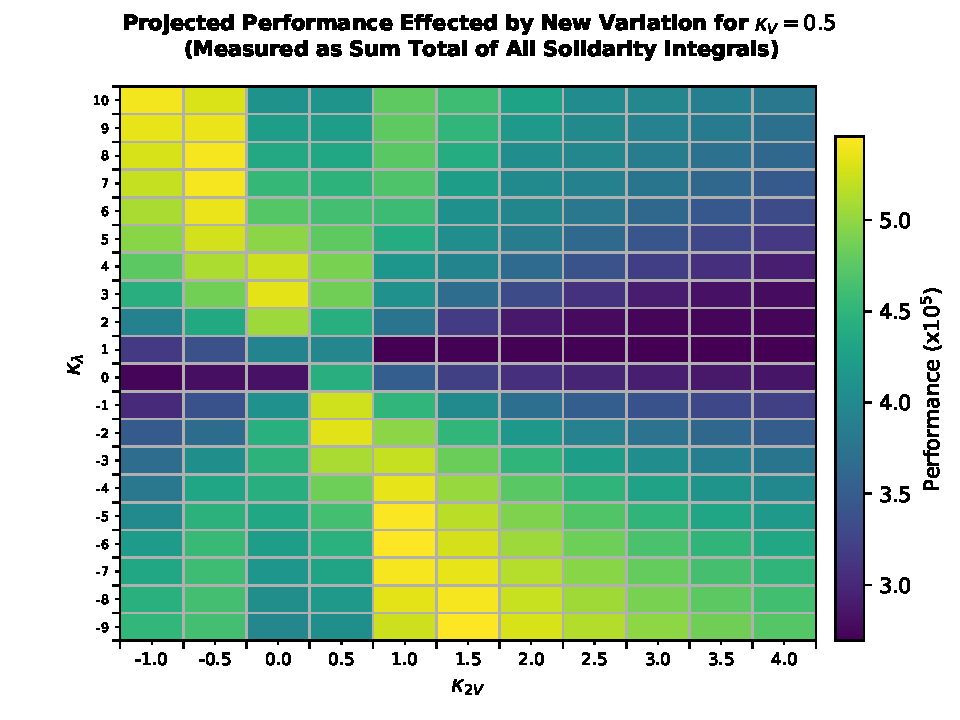
\includegraphics[width=0.5\linewidth,height=\textheight,keepaspectratio]{signal/solidarity_performance_kv0.5}
        }
        \subfloat[\kv = 1.5]{
            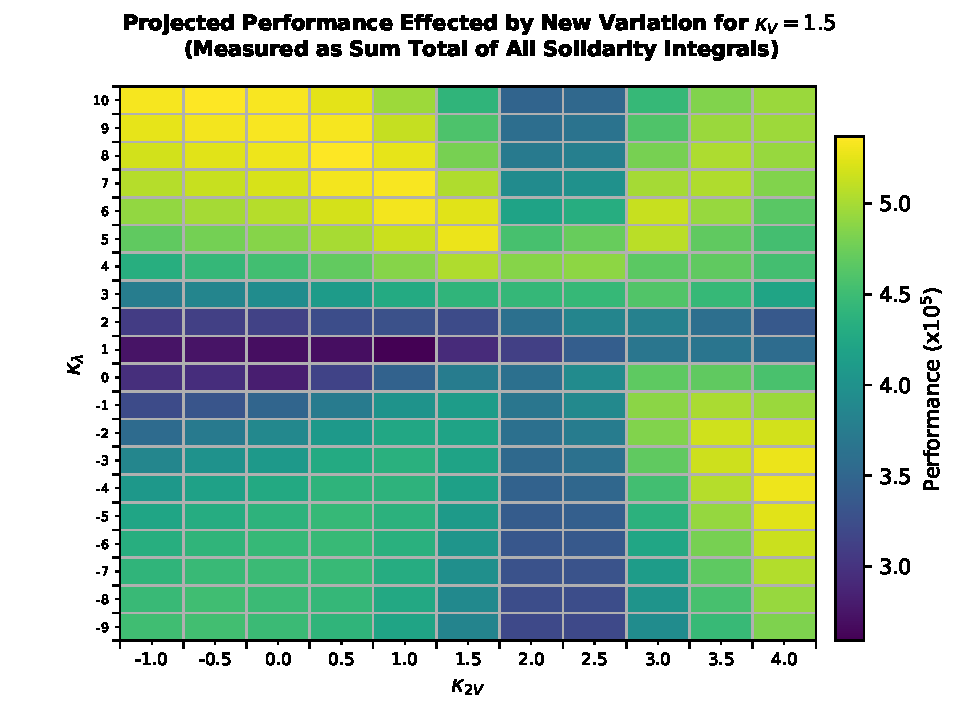
\includegraphics[width=0.5\linewidth,height=\textheight,keepaspectratio]{signal/solidarity_performance_kv1.5}
        }
        \caption{
            Solidarity cumulative performance maps for various values of \kv.
            The color of a particular (\kvv,\kl) point indicates the overall
                benefit to adding an MC sample with that set of couplings
                to the existing set of 12 MC samples.
        }
        \label{fig:solidarity_performance_map}
    \end{figure}

    Using Figure \ref{fig:solidarity_performance_map} as a guide,
        a number of points (mostly those corresponding to the highest aggregate performance values, ~5.5)
        were selected for limited simulation at truth level.
    Based on the prelinary stability shown by these truth level simulations,
        a full MC production run was generated with its coupling values set to \kvv=1, \kl=-5, \kv=0.5.
